\documentclass{article}
\usepackage[sc]{mathpazo}
\usepackage[utf8]{inputenc}
\linespread{1.05}
\usepackage[spanish]{babel}
\usepackage{enumitem}
\setlist[itemize]{noitemsep}
\usepackage{blindtext}
\usepackage{lettrine}
\usepackage[hmarginratio=1:1,top=32mm,columnsep=20pt]{geometry} 
\usepackage{titling}
\usepackage{abstract} % Allows abstract customization
\usepackage{tipa}
\usepackage{graphicx}
\usepackage{listings}
\renewcommand{\abstractnamefont}{\normalfont\bfseries} 
\usepackage{titlesec} % Allows customization of titles
\renewcommand\thesection{\Roman{section}} % Roman numerals for the sections
\renewcommand\thesubsection{\roman{subsection}} % roman numerals for subsections

\setlength{\droptitle}{-4\baselineskip} % Move the title up
\pretitle{\begin{center}\Huge\bfseries} % Article title formatting
\posttitle{\end{center}} % Article title closing formatting
\title{Implementación de Algoritmos Genéticos para Problema de la Cadena más Cercana (CSP)}
\author{
  Diego Carrillo Verduzco \\
  Universidad Nacional Autónoma de México
}
\date{\today}
\renewcommand{\maketitlehookd}{
\begin{abstract}
  Los algoritmos genéticos son heurísticas inspiradas en los mecanísmos de la selección
  natural para resolver problemas de búsqueda y optimización. Con fines didácticos se realizó una
  implementación de esta heurística orientada hacia encontrar soluciones de instancias del problema
  de la cadena más cercana (CSP) con el fin de encontrar su efectividad a través de experimentación.
  Se encontraron resultados adecuados acerca de la heurística y realidades incómodas sobre la generación
  aleatoria de instancias del problema.
\end{abstract}
}
\begin{document}
\maketitle
\section{Introducción}
  El propósito de este documento es presentar una visión general de los algoritmos genéticos, describir
  brevemente su proceso de implementación y discutir su efectividad al utilizarlos para taclear el problema
  de la cadena más cercana. Adicionalmente, se describe este problema y se interroga la fiabilidad de 
  generar instancias de él aleatoriamente para propósitos de experimentación.

\section{La Heurística}
  Un algoritmo genético es una metaheurística inspirada por el proceso de selección natural, utilizada
  para generar soluciones a problemas de búsqueda y optimización.

  Para utilizar un algorítmo genético para encontrar soluciones a un problema, primero es necesario 
  encontrar una representación \textit{cromosómica} o \textit{genotípica} de la solución; típicamente
  esto implica encontrar una representación en cadenas binarias de 1s y 0s, pero la codificación no tiene
  que ser necesariamente de esa forma, basta con que la codificación encapsule apropiadamente las características 
  de la solución.
  
  En segundo lugar, se ha de establecer una función de \textit{aptitud}, que determine la calidad de cierta
  solución. En problemas de optimización, esta aptitud puede ser la función objetivo que se intenta resolver.

  Al iniciar el algoritmo genético, se tiene una población de \textit{individuos} (soluciones candidatas)
  de entre los cuales se debe seleccionar estocásticamente para engendrar una nueva generación de individuos.
  Usualmente, el proceso de selección debe favorecer a los individuos con mayor aptitud, de tal manera que se
  preserven las propiedades de esos individuos; sin embargo se pueden seleccionar diversas formas de seleccionar 
  a los individuos.

  Una vez habiendo seleccionado a los candidatos para engendrar la siguiente generación, se aplican una serie de 
  \textit{operadores genéticos}. Entre estos se encuentran: 
  \begin{enumerate}
    \item \textbf{Recombinación}: En este operador se combina la información de los cromosomas de dos o más
      individuos diferentes, creando por lo menos un nuevo individuo con carácterísticas de los individuos "padres".
      Usualmente, si se ve la representación genotípica de la solución como un arreglo de bits, la recombinación
      se efectúa escogiendo un índice del arreglo y copiando la información del individuo $A$ al nuevo individuo
      hasta ese índice, y después de ese índice se copia la información del individuo $B$ al nuevo individuo.

    \item \textbf{Mutación}: Con este operador se selecciona al azar alguno de los genes de una solución y se cambia
      aleatoriamente a otro valor. Por ejemplo, si la representación genética fuera una cadena de bits, la mutación
      representaría escoger un bit al azar de la cadena y voltearlo a su valor opuesto.
  \end{enumerate}
  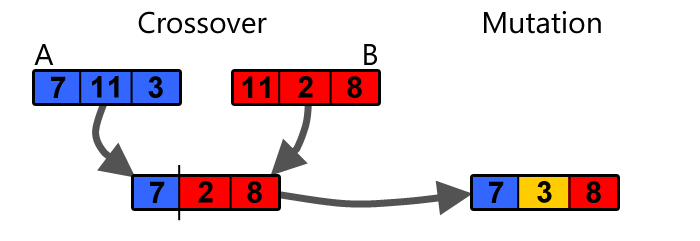
\includegraphics[width=\textwidth]{crossover_mutation}
  Se aplican estos operadores sobre la poblacion actual hasta obtener suficientes individuos nuevos para llenar 
  una generación nueva. Se reemplaza la población anterior con la recientemente generada y se repite iterativamente este
  proceso hasta que se cumpla alguna condición de término. Entre estas condiciones de término podemos considerar llegar a
  un número predeterminado de generaciones creadas, alcanzar la solución de máxima aptitud posible (si es que ésta se 
  conoce), alcanzar el límite de recursos asignados al proceso, etcétera.

\section{El Problema}
  El problema de la cadena más cercana (CSP, por sus siglas en inglés: Closest String Problem) consiste
  en lo siguiente: dado un conjunto de cadenas $S$ de longitud $L$, encontrar una cadena $s$ tal que 
  la máxima distancia entre $s$ y todas las cadenas en $S$ sea la mínima posible, en donde la distancia 
  entre dos cadenas $s$ y $p$ es la distancia de Hamming, la cual se puede definir recursivamente 
  así (viendo las cadenas como listas de caracteres):
  \begin{lstlisting}
    hamming :: String -> String -> Int
    hamming [] _ = 0
    hamming _ [] = 0
    hamming (x:s) (y:p) = if (x != y) then 
                              1 + (hamming s p) 
                          else 
                              (hamming s p)
  \end{lstlisting}
  Es decir, cuenta la cantidad de veces que el $i$-ésimo caracter de la cadena s es diferente del $i$-esimo
  caracter de la cadena p.

  Para cualquier conjunto de cadenas de longitud $L$, la máxima distancia posible de cualquier cadena a todas 
  las cadenas del conjunto es $L$, y la mínima posible es 0 (lo cual solamente es posible si todas las 
  cadenas del conjunto son iguales).

  Es posible normalizar el conjunto de cadenas de entrada para reducir el tamaño del alfabeto sobre el que se ha
  de buscar. Si vemos las cadenas como una matriz en donde la $i$-ésima columna representa el $i$-ésimo caracter
  de todas las cadenas, reemplazamos el caracter más frecuente de la columna con un 0 (o algún otro símbolo), al segundo más
  frecuente con un 1, y así sucesivamente. Esto limita el tamaño del alfabeto a, a lo más, la cantidad de cadenas 
  del conjunto.

\section{La Implementación}
  Para la implementación del algoritmo genético se utilizó el lenguaje de programación \textbf{Rust} por una variedad
  de razones. Para conocer estas razones, refiérase al documento de reporte del proyecto \textit{Implementación de Recocido
  Simulado para Problema del Agente Viajero}.

  La estructura del proyecto se separa en módulos, cada uno de los cuales tiene una función específica:
  \begin{enumerate}
    \item \textbf{normalizer.rs} - normaliza el conjunto de cadenas de entrada para limitar el espacio de búsqueda
      para las soluciones.
    \item \textbf{solution.rs} - codifica las representación de las cadenas solución como arreglos de números enteros 
      y contiene la implementación de las soluciones y todos sus métodos relevantes: distancia, costo, etc.
    \item \textbf{population.rs} - representa la población de soluciones e implementa los métodos necesarios para
      realizar el proceso de evolución: selección aleatoria y generación de individuos nuevos.
    \item \textbf{main-rs} - lee el archivo de configuración y utiliza el módulo Population para empezar el proceso
      del algoritmo genético.
  \end{enumerate}
\section{La experimentación}
  Existen diversos parámetros para la ejecución de un algoritmo genético que no están determinados. Estos parámetros,
  por supuesto, están sujetos a ser manipulados durante la búsqueda de soluciones para encontrar qué configuraciones
  resultan en los mejores resultados al experimentar. Los parámetros configurables del programa se encuentran en el archivo 
  \textbf{Settings.toml} y son:
  \begin{itemize}
    \item \textbf{seeds} - lista de semillas del generador de números aleatorios. Cada semilla resulta en una ejecución 
      del algoritmo.
    \item \textbf{pop\_size} - tamaño de la población de individuos.
    \item \textbf{generations} - cantidad de generaciones que deben engendrarse antes de que la ejecución del algoritmo se detenga.
    \item \textbf{from\_init} - determina si los individuos iniciales se toman del conjunto de cadenas de entrada. Si su valor
      es \textit{false}, los individuos iniciales se generan aleatoriamente.
    \item \textbf{mut\_prob} - probabilidad de que un individuo recién nacido de la recombinación de otros dos mute alguno
      de sus genes aleatoriamente. Una probabilidad muy alta tiende a degenerar las soluciones hacia el final de la ejecución,
      empeorando la aptitud de las soluciones.
  \end{itemize}
\section{Los Resultados}
  Un obstáculo importante que se descubrió al intentar generar conjuntos de cadenas aleatorias para experimentar fue que
  bajo ciertas circunstancias, puede llegar a ser muy fácil que el conjunto no tenga cadenas 'centrales', esto es, que 
  exista una cadena con distancia a todas las cadenas menor que la máxima (o sea, la longitud de las cadenas).
  Por esta razón fue necesario construir conjuntos de entrada de manera que las cadenas estuvieran 'cercanas' entre sí,
  lo cual se logró generando una cadena aleatoria que actuara como 'centro' y a partir de ella generar más cadenas
  aleatorias cambiando una cantidad acotada superiormente de caracteres de esa cadena.

  Se hicieron pruebas con un conjunto de 500 cadenas de longitud 100 con distancia máxima entre ellas de 50.
  Con 10 semillas diferentes, con tamaños de poblacion de 500, 1000 y 2000, con 2000 y 3000 generaciones máximas,
  e inicializando las cadenas a partir del conjunto de entrada o aleatoriamente, con 33\% probabilidad de
  mutación, se obtuvo siempre una cadena con distancia máxima 31. El único parámetro con impacto
  significativo sobre la calidad de la mejor cadena generada fue la probabilidad de mutación. Al hacer pruebas
  con 50\% y 75\% probabilidad de mutación, la mejor solución generada tuvo distancias de 33 y 34 respectivamente.

\section{Las Conclusiones}
  La implementación del proyecto sugiere que, dado un conjunto de entrada que represente un problema verdadero
  y no una instancia generada aleatoriamente, el uso de algoritmos genéticos podría ser muy efectivo para generar soluciones
  al problema de la cadena más cercana. Aunque la experimentación no fue extensa, los resultados mostraban potencial.

  El uso de algoritmos genéticos parece poder mejorarse utilizando algún preprocedimiento que permita generar 
  soluciones de calidad decente antes de empezar el proceso evolutivo. Por ejemplo, un preprocedimiento que utilizara
  recocido simulado para generar una cantidad de soluciones de calidad aceptable para utilizar como individuos iniciales
  podría quizás aumentar la calidad final de las soluciones encontradas.

\section{Bibliografía}
  \begin{enumerate}
    \item Mitchell, M. (1998). \textit{An Introduction to Genetic Algorithms.} The MIT Press.
    \item Chimani, M., Woste M., Böcker, S. (2011). \textit{A Closer Look at the Closest String and Closest Substring Problem}. 
  \end{enumerate}
\end{document}
